\chapter[Análisis]{
  \label{chp:analisis}
  ANÁLISIS
}
\thispagestyle{numberingStyle}
\pagestyle{numberingStyle}

En este apartado se explicará, detalladamente, el análisis realizado.

\section{Análisis de requerimientos}

\subsection{Requerimientos funcionales}
A continuación se muestran los requerimientos funcionales del sistema, clasificados en distintas áreas.

\subsubsection*{Acceso a la aplicación}
\begin{itemize}
\setlength\itemsep{1pt}
\item El sistema ofrecerá la posibilidad de que un usuario se registre en la aplicación.
\item El sistema ofrecerá la posibilidad de que el usuario se identifique en el sistema. Los usuarios deben ingresar al sistema con  nombre de usuario y contraseña.
\end{itemize}

\subsubsection*{Cliente Móvil}
\begin{itemize}
\setlength\itemsep{1pt}
\item El sistema ofrecerá la posibilidad de crear nuevas rutas.
\item El usuario podrá consultar las rutas, propias y de otros usuarios, según ciertos criterios de búsqueda.
\item El sistema permitirá a los usuarios autorizados eliminar las rutas propias que deseen.
\item El sistema permitirá a los usuarios autorizados a consultar los detalles de las rutas.
\item Para las rutas, el sistema permitirá:
	\begin{itemize}
	\item Establecer las fechas de inicio y fin.
	\item Consultar, asignar y desasignar a la ruta, los eventos disponibles en esas fechas.
	\item Consultar el itinerario por días.
	\item Modificar la hora de comienzo establecida para cada día.
	\item Consultar, añadir y eliminar lugares de interés a cada día de la ruta.
	\item Editar el modo de viaje a realizar entre diferentes lugares.
	\item Mostrar el itinerario, por días y en total, en el mapa.
	\item Habilitar y deshabilitar el sistema de geolocalización para conocer la ruta hecha en tiempo real.
	\item Consultar y comparar, el itinerario definido con el obtenido a tiempo real.
	\item Editar los permisos de la ruta.
	\end{itemize}
\end{itemize}

\subsubsection*{Cliente Web}
\begin{itemize}
\setlength\itemsep{1pt}
\item El usuario podrá consultar las rutas existentes, propias y de otros usuarios, según ciertos criterios de búsqueda.
\item El sistema permitirá a los usuarios autorizados a consultar los detalles de las rutas.
\item El sistema permitirá a los usuarios autorizados marcar las rutas propias como privadas, con el fin de no compartirlas con los demás usuarios.
\item El sistema solo ofrecerá la posibilidad de consulta sobre los detalles de una ruta, permitiendo ver el itinerario, si tiene datos en tiempo real guardados, etc...
\item El sistema permitirá a los usuarios autorizados eliminar las rutas propias que deseen.
\end{itemize}

\subsubsection*{Cliente Administración Web}
\begin{itemize}
\setlength\itemsep{1pt}
\item El sistema solo permitirá acceso a usuarios con permisos de administración.
\item El sistema permitirá a los usuarios con dichos permisos, dar de alto nuevos usuarios.
\item El sistema permitirá las altas, bajas, modificaciones y consultas de las entidades del sistema.
	\begin{itemize}
	\item El sistema ofrecerá la posibilidad de crear, eliminar, modificar y consultar datos de usuarios.
	\item El sistema ofrecerá la posibilidad de crear, eliminar, modificar y consultar datos de rutas.
	\item El sistema ofrecerá la posibilidad de crear, eliminar, modificar y consultar datos de lugares.
	\item El sistema ofrecerá la posibilidad de crear, eliminar, modificar y consultar datos de categorías.
	\item El sistema ofrecerá la posibilidad de crear, eliminar, modificar y consultar datos de eventos.
	\end{itemize}
\item El sistema permitirá la existencia de usuarios con capacidades para la administración y gestión, exclusivamente, de los eventos. Permitiendo así, sus altas,  bajas, modificaciones y consultas de los mismos en el sistema.
\end{itemize}

\subsubsection*{Seguridad}
\begin{itemize}
\setlength\itemsep{1pt}
\item El sistema ofrecerá la posibilidad de que el usuario modifique sus datos de acceso al sistema.
\item El sistema solo permitirá acciones correctamente autenticadas, exceptuando las de acceso a la aplicación.
\item Los usuarios de la aplicación solo podrán modificar los datos a los que el usuario esté autorizado. Un usuario no podrá modificar la información de los recursos de los que no es propietario.
\item Los intercambios de datos que realice el sistema a través de internet, serán mediante el uso del protocolo encriptado https.
\end{itemize}


\subsection{Requerimientos no funcionales}





\section{Modelo de casos de uso}

\subsection{Actores del sistema}
Analizando los requerimientos funcionales funcionales del sistema, se detectan tres tipos de actores, que demandan una determinada funcionalidad en el sistema. Estos tres actores son, el cliente, el administrador y el gestor de eventos.


\begin{figure}[htbp]
\centering
\vspace*{0.2in}
\includesvg{actores.svg}
\caption{Diagrama casos de uso aplicación móvil.}
\end{figure}


\subsection{Diagrama de casos de uso}
Tras conocer los requerimientos funcionales del sistema y reconocer las necesidades del sistema, se ha optado por diseñar un sistema general compuesto por los diferentes subsistemas del mismo.


\FloatBarrier
\subsubsection*{Diagrama sistema general}
Dicho sistema, estará compuesto por tres grupos de subsistemas: subsistema de acceso, subsistema de administración y subsistema de aplicación.

\begin{figure}[!htbp]
\centering

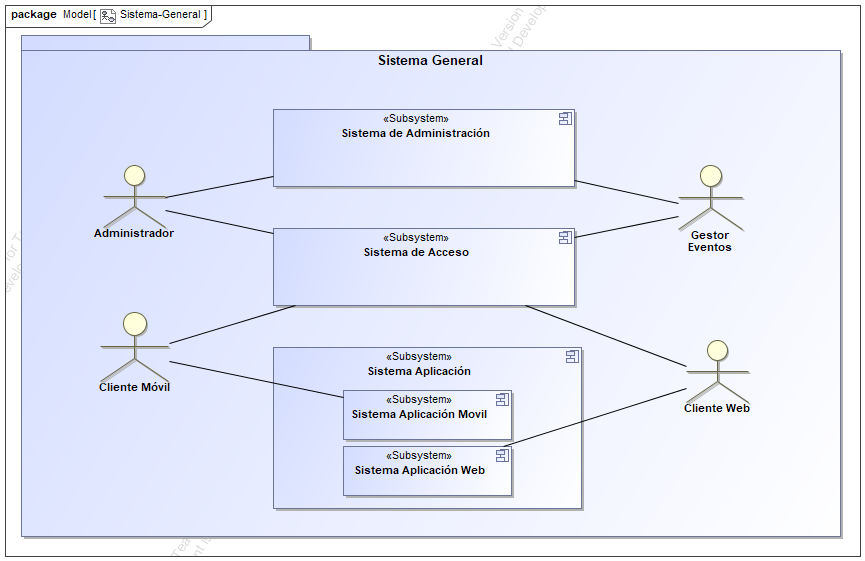
\includegraphics[
   keepaspectratio=true
]{./../Diagrams/uc__Sistema-General.png}
\caption{Diagrama casos de uso - Sistema general.}
\end{figure}


\FloatBarrier
\subsubsection*{Diagrama sistema de acceso}
\begin{figure}[!htbp]
\centering

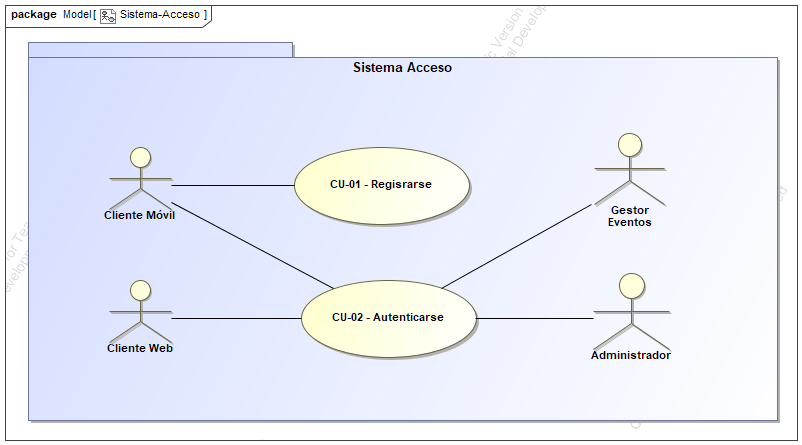
\includegraphics[
   keepaspectratio=true
]{./../Diagrams/uc__Sistema-Acceso.png}
\caption{Diagrama casos de uso - Sistema general.}
\end{figure}


\FloatBarrier
\subsubsection*{Diagrama sistema aplicación móvil}
\begin{figure}[!htbp]
\centering

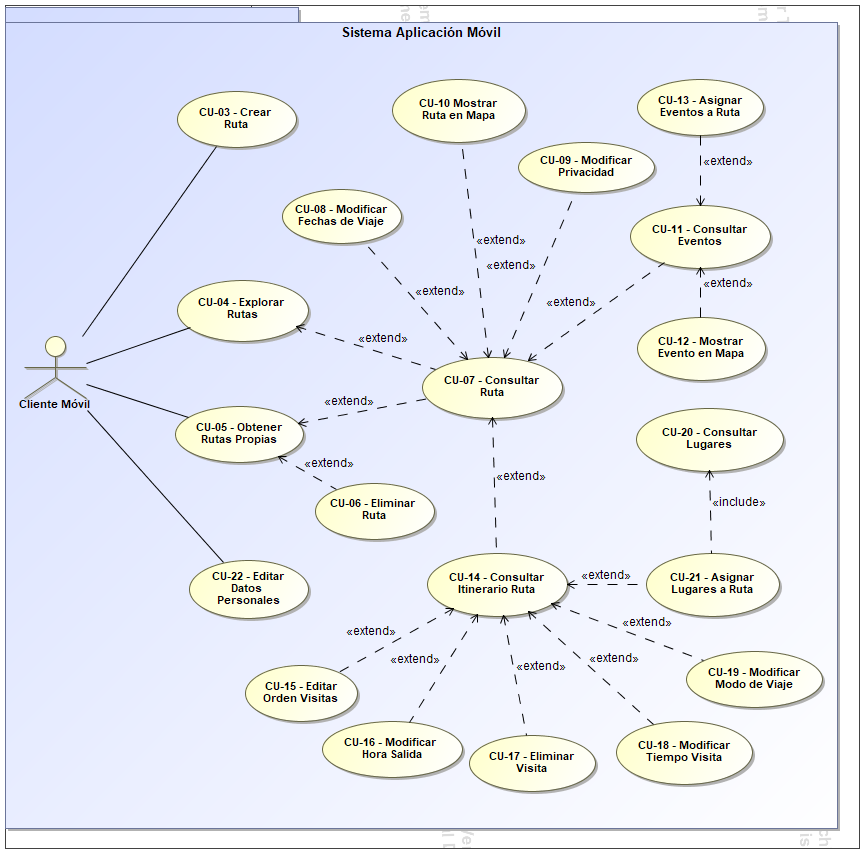
\includegraphics[
   keepaspectratio=true
]{./../Diagrams/Sistema-Aplicacion-Movil.png}
\caption{Diagrama casos de uso - Sistema general.}
\end{figure}


\FloatBarrier
\subsubsection*{Diagrama sistema aplicación web}
\begin{figure}[!htbp]
\centering

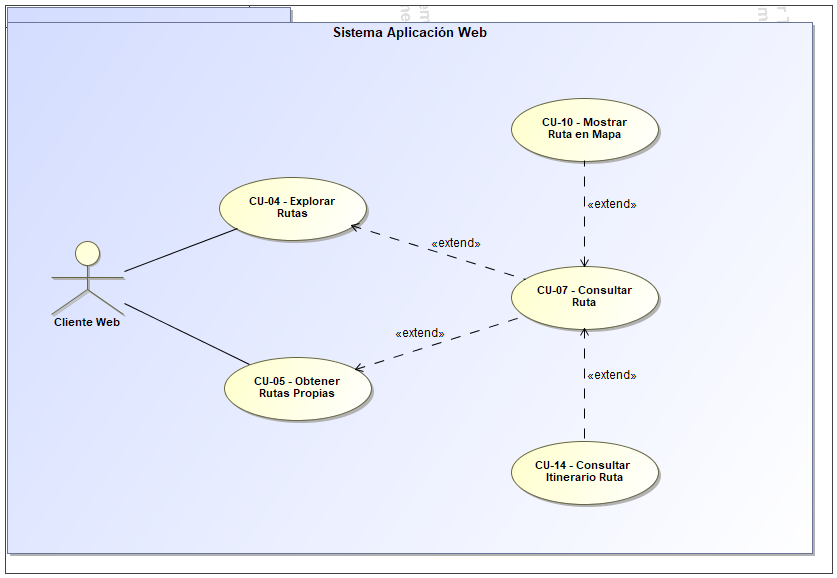
\includegraphics[
   keepaspectratio=true
]{./../Diagrams/Sistema-Aplicacion-Web.png}
\caption{Diagrama casos de uso - Sistema general.}
\end{figure}


\FloatBarrier
\subsubsection*{Diagrama sistema administración}
\begin{figure}[!htbp]
\centering

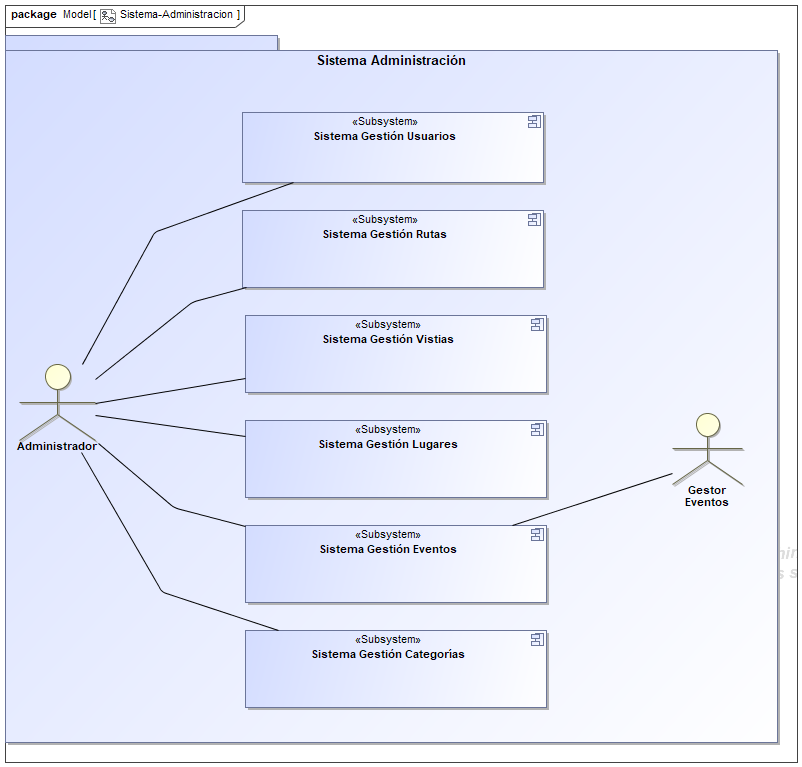
\includegraphics[
   keepaspectratio=true
]{./../Diagrams/Sistema-Administracion.png}
\caption{Diagrama casos de uso - Sistema general.}
\end{figure}


\FloatBarrier
\subsubsection*{Diagrama sistema gestión usuarios}
\begin{figure}[!htbp]
\centering

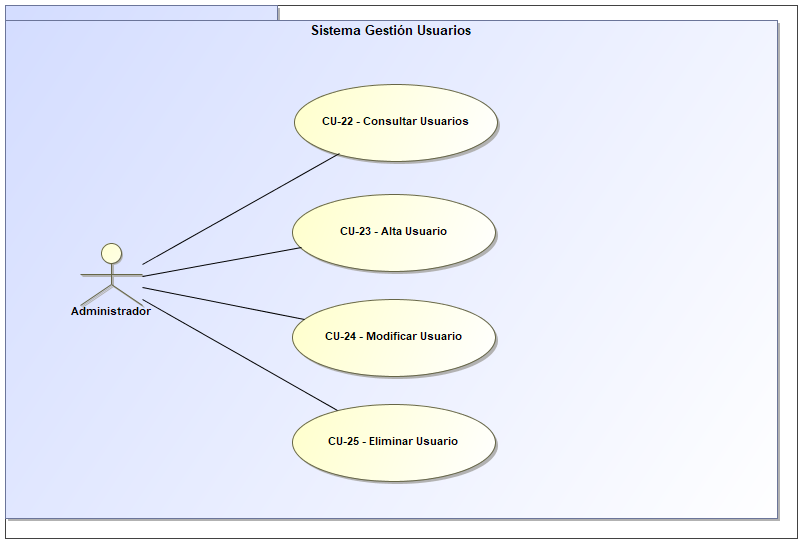
\includegraphics[
   keepaspectratio=true
]{./../Diagrams/Sistema-Gestion-Usuarios.png}
\caption{Diagrama casos de uso - Sistema general.}
\end{figure}


\FloatBarrier
\subsubsection*{Diagrama sistema gestión rutas}
\begin{figure}[!htbp]
\centering

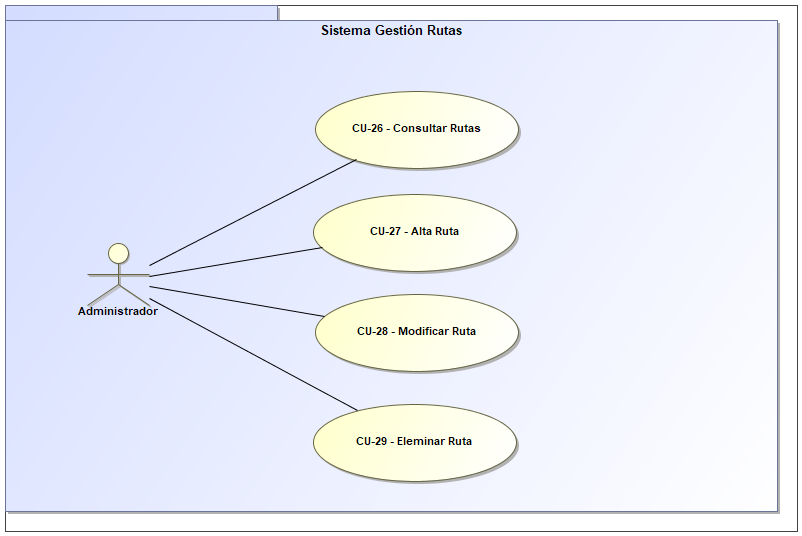
\includegraphics[
   keepaspectratio=true
]{./../Diagrams/Sistema-Gestion-Rutas.png}
\caption{Diagrama casos de uso - Sistema general.}
\end{figure}


\FloatBarrier
\subsubsection*{Diagrama sistema gestión lugares}
\begin{figure}[!htbp]
\centering

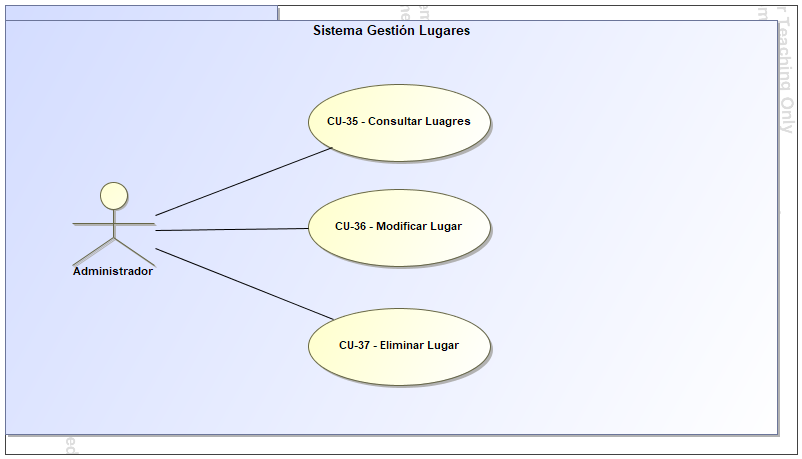
\includegraphics[
   keepaspectratio=true
]{./../Diagrams/Sistema-Gestion-Lugares.png}
\caption{Diagrama casos de uso - Sistema general.}
\end{figure}


\FloatBarrier
\subsubsection*{Diagrama sistema gestión eventos}
\begin{figure}[!htbp]
\centering

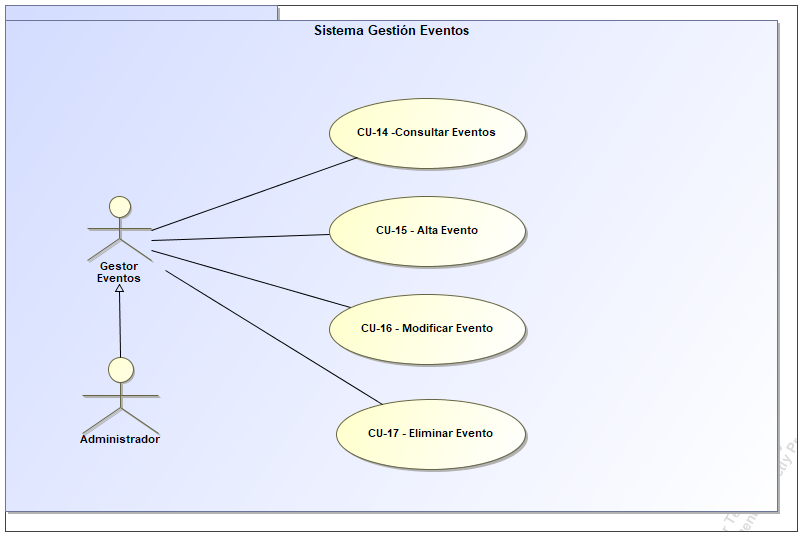
\includegraphics[
   keepaspectratio=true
]{./../Diagrams/Sistema-Gestion-Eventos.png}
\caption{Diagrama casos de uso - Sistema general.}
\end{figure}


\FloatBarrier
\subsubsection*{Diagrama sistema gestión categorías}
\begin{figure}[!htbp]
\centering

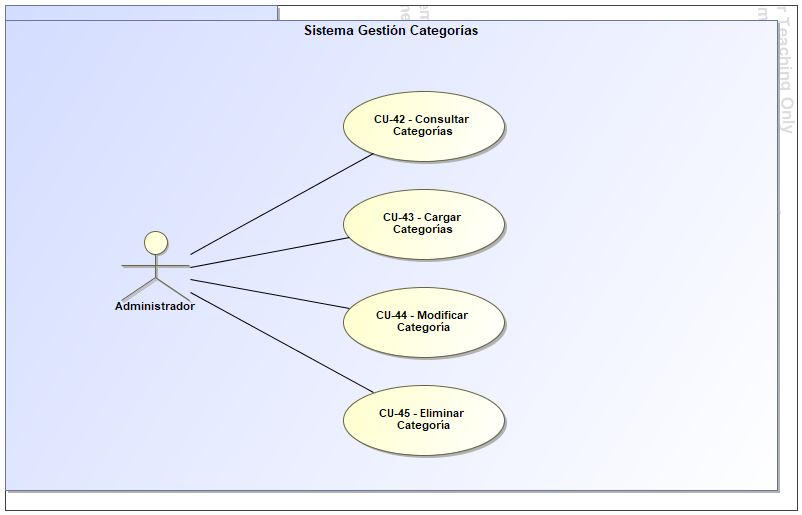
\includegraphics[
   keepaspectratio=true
]{./../Diagrams/Sistema-Gestion-Categorias.png}
\caption{Diagrama casos de uso - Sistema general.}
\end{figure}



\newpage
\subsection{Especificación casos de uso}


\newpage
\subsubsection*{Caso de uso: autenticarse}
\begin{longtable}{| p{4cm} | p{10cm} |}
\endfirsthead
\multicolumn{2}{c}{\textit{Continúa de la página anterior}}\\[12pt]
\hline
\endhead
\hline
\multicolumn{2}{c}{\textit{Continúa en la siguiente página}} \\
\endfoot
\hline
\caption{Caso de Uso: Autenticarse}\label{fig:1}\\
\endlastfoot


\hline
\multicolumn{2}{|c|}{\textbf{CU$<$01$>$ - Autenticarse}} \\

\hline
\textbf{Descripción} &
El usuario se identifica introduciendo las credenciales de acceso en el sistema \\

\hline
\textbf{Actores} &
Cliente Móvil\newline
Cliente Web\newline
Administrador\newline
Moderador\\

\hline
\textbf{Precondiciones} &
N/A\\

\hline
\textbf{Secuencia Normal} &\mbox{}\par\vspace{-\baselineskip}
\begin{enumerate}[leftmargin=0.7cm, topsep=0.1cm]
\item El usuario introduce sus credenciales en la ventana de login. 
\item El usuario pulsa el botón de \textit{Acceder}.
\item El sistema valida las credenciales.
\item El usuario accede a la aplicación.
\end{enumerate}\\

\hline
\textbf{Excepciones} &\mbox{}\par\vspace{-\baselineskip}
\begin{enumerate}[leftmargin=0.9cm, topsep=0.1cm]
\item[3a.] Los datos introducidos no son correctos.
	\begin{itemize}
	\item[1.] El usuario vuelve a introducir las credenciales.
	\end{itemize}

\end{enumerate}\\

\hline
\textbf{Postcondiciones} & 
El usuario queda autenticado en el sistema\\
\hline
\end{longtable}




\newpage
\subsubsection*{Caso de uso: Registrarse}
\begin{longtable}{| p{4cm} | p{10cm} |}
\endfirsthead
\multicolumn{2}{c}{\textit{Continúa de la página anterior}}\\[12pt]
\hline
\endhead
\hline
\multicolumn{2}{c}{\textit{Continúa en la siguiente página}} \\
\endfoot
\hline
\caption{Caso de Uso: Registrarse}\label{fig:1}\\
\endlastfoot


\hline
\multicolumn{2}{|c|}{\textbf{CU$<$02$>$ - Registrarse}} \\

\hline
\textbf{Descripción} &
El usuario introduce los datos para darse de alta en la aplicación. \\

\hline
\textbf{Actores} &
Cliente Móvil\\


\hline
\textbf{Precondiciones} &
N/A\\

\hline
\textbf{Secuencia Normal} &\mbox{}\par\vspace{-\baselineskip}
\begin{enumerate}[leftmargin=0.7cm, topsep=0.1cm]
\item El usuario selecciona la opción de registrarse.
\item El sistema muestra un formulario indicando los campos necesarios para realizar el registro.
\item El usuario rellena los campos y pulsa el botón de \textit{Registrarse}.
\item El sistema valida los datos introducidos por el usuario.
\item El usuario accede a la aplicación.
\end{enumerate}\\

\hline
\textbf{Excepciones} &\mbox{}\par\vspace{-\baselineskip}
\begin{enumerate}[leftmargin=0.9cm, topsep=0.1cm]
\item[3-A.] El usuario pulsa el botón de \textit{Cancelar}.
	\begin{itemize}
	\item[1.] El sistema cancela el registro y redirige al usuario a la pantalla de login.
	\end{itemize}
\item[3-B.] Los datos introducidos por el usuario no son válidos.
	\begin{itemize}
	\item[1.] El sistema muestra un mensaje de error e invita al usuario a volver a introducir los datos. (Regreso al paso 2)
	\end{itemize}
\end{enumerate}\\

\hline
\textbf{Postcondiciones} & 
El usuario queda registrado y autenticado en el sistema\\
\hline
\end{longtable}




\newpage
\subsubsection*{Caso de uso: Crear Ruta}
\begin{longtable}{| p{4cm} | p{10cm} |}
\endfirsthead
\multicolumn{2}{c}{\textit{Continúa de la página anterior}}\\[12pt]
\hline
\endhead
\hline
\multicolumn{2}{c}{\textit{Continúa en la siguiente página}} \\
\endfoot
\hline
\caption{Caso de Uso: Crear Ruta}\label{fig:1}\\
\endlastfoot


\hline
\multicolumn{2}{|c|}{\textbf{CU$<$03$>$ - Crear Ruta}} \\

\hline
\textbf{Descripción} &
El usuario crea una ruta para una ciudad o lugar especificado. \\

\hline
\textbf{Actores} &
Cliente Móvil\\

\hline
\textbf{Precondiciones} &
El usuario está autenticado en la aplicación\\

\hline
\textbf{Secuencia Normal} &\mbox{}\par\vspace{-\baselineskip}
\begin{enumerate}[leftmargin=0.7cm, topsep=0.1cm]
\item El usuario selecciona la opción de crear una nueva ruta.
\item El sistema muestra buscador para que el usuario indique en qué ciudad o lugar desea crear dicha ruta.
\item El usuario rellena el buscador.
\item El sistema ayuda al usuario autocompletando con los datos de diferentes ciudades y lugares.
\item El usuario selecciona el lugar en la lista de autocompletado ofrecida por el sistema.
\item El sistema muestra un mapa indicando la ubicación del lugar seleccionado y permite al usuario completar el proceso de creación.
\item El usuario pulsa el botón para crear la ruta.
\end{enumerate}\\

\hline
\textbf{Excepciones} &\mbox{}\par\vspace{-\baselineskip}
\\

\hline
\textbf{Postcondiciones} & 
La ruta queda registrada en el sistema\\
\hline
\end{longtable}




\newpage
\subsubsection*{Caso de uso: Explorar Rutas}
\begin{longtable}{| p{4cm} | p{10cm} |}
\endfirsthead
\multicolumn{2}{c}{\textit{Continúa de la página anterior}}\\[12pt]
\hline
\endhead
\hline
\multicolumn{2}{c}{\textit{Continúa en la siguiente página}} \\
\endfoot
\hline
\caption{Caso de Uso: Explorar Rutas}\label{fig:1}\\
\endlastfoot


\hline
\multicolumn{2}{|c|}{\textbf{CU$<$04$>$ - Explorar Rutas}} \\

\hline
\textbf{Descripción} &
El usuario explora las diferentes rutas creadas por los demás usuarios.\\

\hline
\textbf{Actores} &
Cliente Móvil\newline
Cliente Web\\

\hline
\textbf{Precondiciones} &
El usuario está autenticado en la aplicación\\

\hline
\textbf{Secuencia Normal} &\mbox{}\par\vspace{-\baselineskip}
\begin{enumerate}[leftmargin=0.7cm, topsep=0.1cm]
\item El usuario selecciona la opción de explorar rutas.
\item El sistema muestra las diferentes rutas que hay en el sistema.
\end{enumerate}\\

\hline
\textbf{Excepciones} &\mbox{}\par\vspace{-\baselineskip}
\\

\hline
\textbf{Postcondiciones} & 
\\
\hline
\end{longtable}



\newpage
\subsubsection*{Caso de uso: Obtener Rutas Propias}
\begin{longtable}{| p{4cm} | p{10cm} |}
\endfirsthead
\multicolumn{2}{c}{\textit{Continúa de la página anterior}}\\[12pt]
\hline
\endhead
\hline
\multicolumn{2}{c}{\textit{Continúa en la siguiente página}} \\
\endfoot
\hline
\caption{Caso de Uso: Obtener Rutas Propias}\label{fig:1}\\
\endlastfoot


\hline
\multicolumn{2}{|c|}{\textbf{CU$<$05$>$ - Obtener Rutas Propias}} \\

\hline
\textbf{Descripción} &
El usuario obtiene las rutas creadas por él.\\

\hline
\textbf{Actores} &
Cliente Móvil\newline
Cliente Web\\

\hline
\textbf{Precondiciones} &
El usuario está autenticado en la aplicación\\

\hline
\textbf{Secuencia Normal} &\mbox{}\par\vspace{-\baselineskip}
\begin{enumerate}[leftmargin=0.7cm, topsep=0.1cm]
\item El usuario selecciona la opción de obtener rutas propias.
\item El sistema muestra las rutas que tiene almacenadas en el sistema y.
\item El sistema clasifica las rutas del usuario en función de su progreso; las que aún no empezaron, las que están en curso y las que ya se realizaron.
\item El usuario selecciona una de las posibilidades ofrecidas por el sistema.
\item El sistema filtra las rutas del usuario según lo solicitado.
\end{enumerate}\\

\hline
\textbf{Excepciones} &\mbox{}\par\vspace{-\baselineskip}
\\

\hline
\textbf{Postcondiciones} & 
\\
\hline
\end{longtable}




\newpage
\subsubsection*{Caso de uso: Consultar Ruta}
\begin{longtable}{| p{4cm} | p{10cm} |}
\endfirsthead
\multicolumn{2}{c}{\textit{Continúa de la página anterior}}\\[12pt]
\hline
\endhead
\hline
\multicolumn{2}{c}{\textit{Continúa en la siguiente página}} \\
\endfoot
\hline
\caption{Caso de Uso: Consultar Ruta}\label{fig:1}\\
\endlastfoot


\hline
\multicolumn{2}{|c|}{\textbf{CU$<$06$>$ - Consultar Ruta}} \\

\hline
\textbf{Descripción} &
El usuario obtiene la información detallada de una ruta concreta.\\

\hline
\textbf{Actores} &
Cliente Móvil\newline
Cliente Web\\

\hline
\textbf{Precondiciones} &
\\

\hline
\textbf{Secuencia Normal} &\mbox{}\par\vspace{-\baselineskip}
\begin{enumerate}[leftmargin=0.7cm, topsep=0.1cm]
\item El usuario selecciona una ruta concreta.
\item El sistema obtiene los datos de la ruta.
\item El sistema muestra un panel con los datos detallados de la ruta.
\end{enumerate}\\

\hline
\textbf{Excepciones} &\mbox{}\par\vspace{-\baselineskip}
\begin{enumerate}[leftmargin=0.9cm, topsep=0.1cm]
\item[3.] El usuario pulsa el botón de \textit{Atrás}.
	\begin{itemize}
	\item[1.] El sistema devuelve al usuario a la vista anterior.
	\end{itemize}
\end{enumerate}
\\

\hline
\textbf{Postcondiciones} & 
\\
\hline
\end{longtable}



\newpage
\subsubsection*{Caso de uso: Modificar Fechas de Viaje}
\begin{longtable}{| p{4cm} | p{10cm} |}
\endfirsthead
\multicolumn{2}{c}{\textit{Continúa de la página anterior}}\\[12pt]
\hline
\endhead
\hline
\multicolumn{2}{c}{\textit{Continúa en la siguiente página}} \\
\endfoot
\hline
\caption{Caso de Uso: Modificar Fechas de Viaje}\label{fig:1}\\
\endlastfoot


\hline
\multicolumn{2}{|c|}{\textbf{CU$<$07$>$ - Modificar Fechas de Viaje}} \\

\hline
\textbf{Descripción} &
El usuario selecciona las fechas en las que se realizará la ruta que está planificando.\\

\hline
\textbf{Actores} &
Cliente Móvil\\

\hline
\textbf{Precondiciones} &
\\

\hline
\textbf{Secuencia Normal} &\mbox{}\par\vspace{-\baselineskip}
\begin{enumerate}[leftmargin=0.7cm, topsep=0.1cm]
\item El usuario selecciona la opción de \textit{Seleccionar Fechas}.
\item El sistema muestra una pantalla con las fechas del calendario.
\item El usuario selecciona la fecha de inicio y fin y pulsa el botón de \textit{Aceptar}.
\item El sistema modifica las fechas de la ruta.
\end{enumerate}\\

\hline
\textbf{Excepciones} &\mbox{}\par\vspace{-\baselineskip}
\begin{enumerate}[leftmargin=0.9cm, topsep=0.1cm]
\item[3.] El usuario pulsa el botón de \textit{Cancelar}.
	\begin{itemize}
	\item[1.] El sistema cancela la modificación de las fechas y cierra la pantalla.
	\end{itemize}
\end{enumerate}
\\

\hline
\textbf{Postcondiciones} & 
Las fechas de la ruta quedan actualizadas en el sistema.\\
\hline
\end{longtable}



\newpage
\subsubsection*{Caso de uso: Modificar Privacidad}
\begin{longtable}{| p{4cm} | p{10cm} |}
\endfirsthead
\multicolumn{2}{c}{\textit{Continúa de la página anterior}}\\[12pt]
\hline
\endhead
\hline
\multicolumn{2}{c}{\textit{Continúa en la siguiente página}} \\
\endfoot
\hline
\caption{Caso de Uso: Modificar Privacidad}\label{fig:1}\\
\endlastfoot


\hline
\multicolumn{2}{|c|}{\textbf{CU$<$08$>$ - Modificar Privacidad}} \\

\hline
\textbf{Descripción} &
El usuario puede alternar la privacidad de cada una de sus rutas permitiendo que sean visible para todos o solo para él.\\

\hline
\textbf{Actores} &
Cliente Móvil\\

\hline
\textbf{Precondiciones} &
\\

\hline
\textbf{Secuencia Normal} &\mbox{}\par\vspace{-\baselineskip}
\begin{enumerate}[leftmargin=0.7cm, topsep=0.1cm]
\item El usuario selecciona la opción de \textit{Detalles de la Ruta}.
\item El sistema muestra una pantalla con los detalles de la ruta.
\item El sistema incluye un botón que permite alternar entre los estados de privacidad.
\item El usuario pulsa el botón.
\item El sistema cambia el valor del botón y actualiza el nuevo valor de privacidad.
\end{enumerate}\\

\hline
\textbf{Excepciones} &\mbox{}\par\vspace{-\baselineskip}
\begin{enumerate}[leftmargin=0.9cm, topsep=0.1cm]
\item[4.] El usuario pulsa el botón de \textit{Cancelar}.
	\begin{itemize}
	\item[1.] El sistema retorna a la pantalla anterior.
	\end{itemize}
\end{enumerate}
\\

\hline
\textbf{Postcondiciones} & 
La privacidad de la ruta queda actualizada.\\
\hline
\end{longtable}



\newpage
\subsubsection*{Caso de uso: Mostrar Ruta en Mapa}
\begin{longtable}{| p{4cm} | p{10cm} |}
\endfirsthead
\multicolumn{2}{c}{\textit{Continúa de la página anterior}}\\[12pt]
\hline
\endhead
\hline
\multicolumn{2}{c}{\textit{Continúa en la siguiente página}} \\
\endfoot
\hline
\caption{Caso de Uso: Mostrar Ruta en Mapa}\label{fig:1}\\
\endlastfoot


\hline
\multicolumn{2}{|c|}{\textbf{CU$<$09$>$ - Mostrar Ruta en Mapa}} \\

\hline
\textbf{Descripción} &
El usuario puede mostrar la información de la ruta en el mapa.\\

\hline
\textbf{Actores} &
Cliente Móvil\newline
Cliente Web\\

\hline
\textbf{Precondiciones} &
\\

\hline
\textbf{Secuencia Normal} &\mbox{}\par\vspace{-\baselineskip}
\begin{enumerate}[leftmargin=0.7cm, topsep=0.1cm]
\item El usuario selecciona la opción de \textit{Mostrar Ruta en Mapa}.
\item El sistema muestra un mapa con las marcas de los lugares indicados en un día concreto de la ruta.
\item El usuario puede cambiar entre los días haciendo click sobre ellos.
\end{enumerate}\\

\hline
\textbf{Excepciones} &\mbox{}\par\vspace{-\baselineskip}
\begin{enumerate}[leftmargin=0.9cm, topsep=0.1cm]
\item[3.] El usuario pulsa el botón de \textit{Cancelar}.
	\begin{itemize}
	\item[1.] El sistema retorna a la pantalla anterior.
	\end{itemize}
\end{enumerate}
\\

\hline
\textbf{Postcondiciones} & 
La privacidad de la ruta queda actualizada.\\
\hline
\end{longtable}